\documentclass[1p]{elsarticle_modified}
%\bibliographystyle{elsarticle-num}

%\usepackage[colorlinks]{hyperref}
%\usepackage{abbrmath_seonhwa} %\Abb, \Ascr, \Acal ,\Abf, \Afrak
\usepackage{amsfonts}
\usepackage{amssymb}
\usepackage{amsmath}
\usepackage{amsthm}
\usepackage{scalefnt}
\usepackage{amsbsy}
\usepackage{kotex}
\usepackage{caption}
\usepackage{subfig}
\usepackage{color}
\usepackage{graphicx}
\usepackage{xcolor} %% white, black, red, green, blue, cyan, magenta, yellow
\usepackage{float}
\usepackage{setspace}
\usepackage{hyperref}

\usepackage{tikz}
\usetikzlibrary{arrows}

\usepackage{multirow}
\usepackage{array} % fixed length table
\usepackage{hhline}

%%%%%%%%%%%%%%%%%%%%%
\makeatletter
\renewcommand*\env@matrix[1][\arraystretch]{%
	\edef\arraystretch{#1}%
	\hskip -\arraycolsep
	\let\@ifnextchar\new@ifnextchar
	\array{*\c@MaxMatrixCols c}}
\makeatother %https://tex.stackexchange.com/questions/14071/how-can-i-increase-the-line-spacing-in-a-matrix
%%%%%%%%%%%%%%%

\usepackage[normalem]{ulem}

\newcommand{\msout}[1]{\ifmmode\text{\sout{\ensuremath{#1}}}\else\sout{#1}\fi}
%SOURCE: \msout is \stkout macro in https://tex.stackexchange.com/questions/20609/strikeout-in-math-mode

\newcommand{\cancel}[1]{
	\ifmmode
	{\color{red}\msout{#1}}
	\else
	{\color{red}\sout{#1}}
	\fi
}

\newcommand{\add}[1]{
	{\color{blue}\uwave{#1}}
}

\newcommand{\replace}[2]{
	\ifmmode
	{\color{red}\msout{#1}}{\color{blue}\uwave{#2}}
	\else
	{\color{red}\sout{#1}}{\color{blue}\uwave{#2}}
	\fi
}

\newcommand{\Sol}{\mathcal{S}} %segment
\newcommand{\D}{D} %diagram
\newcommand{\A}{\mathcal{A}} %arc


%%%%%%%%%%%%%%%%%%%%%%%%%%%%%5 test

\def\sl{\operatorname{\textup{SL}}(2,\Cbb)}
\def\psl{\operatorname{\textup{PSL}}(2,\Cbb)}
\def\quan{\mkern 1mu \triangleright \mkern 1mu}

\theoremstyle{definition}
\newtheorem{thm}{Theorem}[section]
\newtheorem{prop}[thm]{Proposition}
\newtheorem{lem}[thm]{Lemma}
\newtheorem{ques}[thm]{Question}
\newtheorem{cor}[thm]{Corollary}
\newtheorem{defn}[thm]{Definition}
\newtheorem{exam}[thm]{Example}
\newtheorem{rmk}[thm]{Remark}
\newtheorem{alg}[thm]{Algorithm}

\newcommand{\I}{\sqrt{-1}}
\begin{document}

%\begin{frontmatter}
%
%\title{Boundary parabolic representations of knots up to 8 crossings}
%
%%% Group authors per affiliation:
%\author{Yunhi Cho} 
%\address{Department of Mathematics, University of Seoul, Seoul, Korea}
%\ead{yhcho@uos.ac.kr}
%
%
%\author{Seonhwa Kim} %\fnref{s_kim}}
%\address{Center for Geometry and Physics, Institute for Basic Science, Pohang, 37673, Korea}
%\ead{ryeona17@ibs.re.kr}
%
%\author{Hyuk Kim}
%\address{Department of Mathematical Sciences, Seoul National University, Seoul 08826, Korea}
%\ead{hyukkim@snu.ac.kr}
%
%\author{Seokbeom Yoon}
%\address{Department of Mathematical Sciences, Seoul National University, Seoul, 08826,  Korea}
%\ead{sbyoon15@snu.ac.kr}
%
%\begin{abstract}
%We find all boundary parabolic representation of knots up to 8 crossings.
%
%\end{abstract}
%\begin{keyword}
%    \MSC[2010] 57M25 
%\end{keyword}
%
%\end{frontmatter}

%\linenumbers
%\tableofcontents
%
\newcommand\colored[1]{\textcolor{white}{\rule[-0.35ex]{0.8em}{1.4ex}}\kern-0.8em\color{red} #1}%
%\newcommand\colored[1]{\textcolor{white}{ #1}\kern-2.17ex	\textcolor{white}{ #1}\kern-1.81ex	\textcolor{white}{ #1}\kern-2.15ex\color{red}#1	}

{\Large $\underline{12a_{0186}~(K12a_{0186})}$}

\setlength{\tabcolsep}{10pt}
\renewcommand{\arraystretch}{1.6}
\vspace{1cm}\begin{tabular}{m{100pt}>{\centering\arraybackslash}m{274pt}}
\multirow{5}{120pt}{
	\centering
	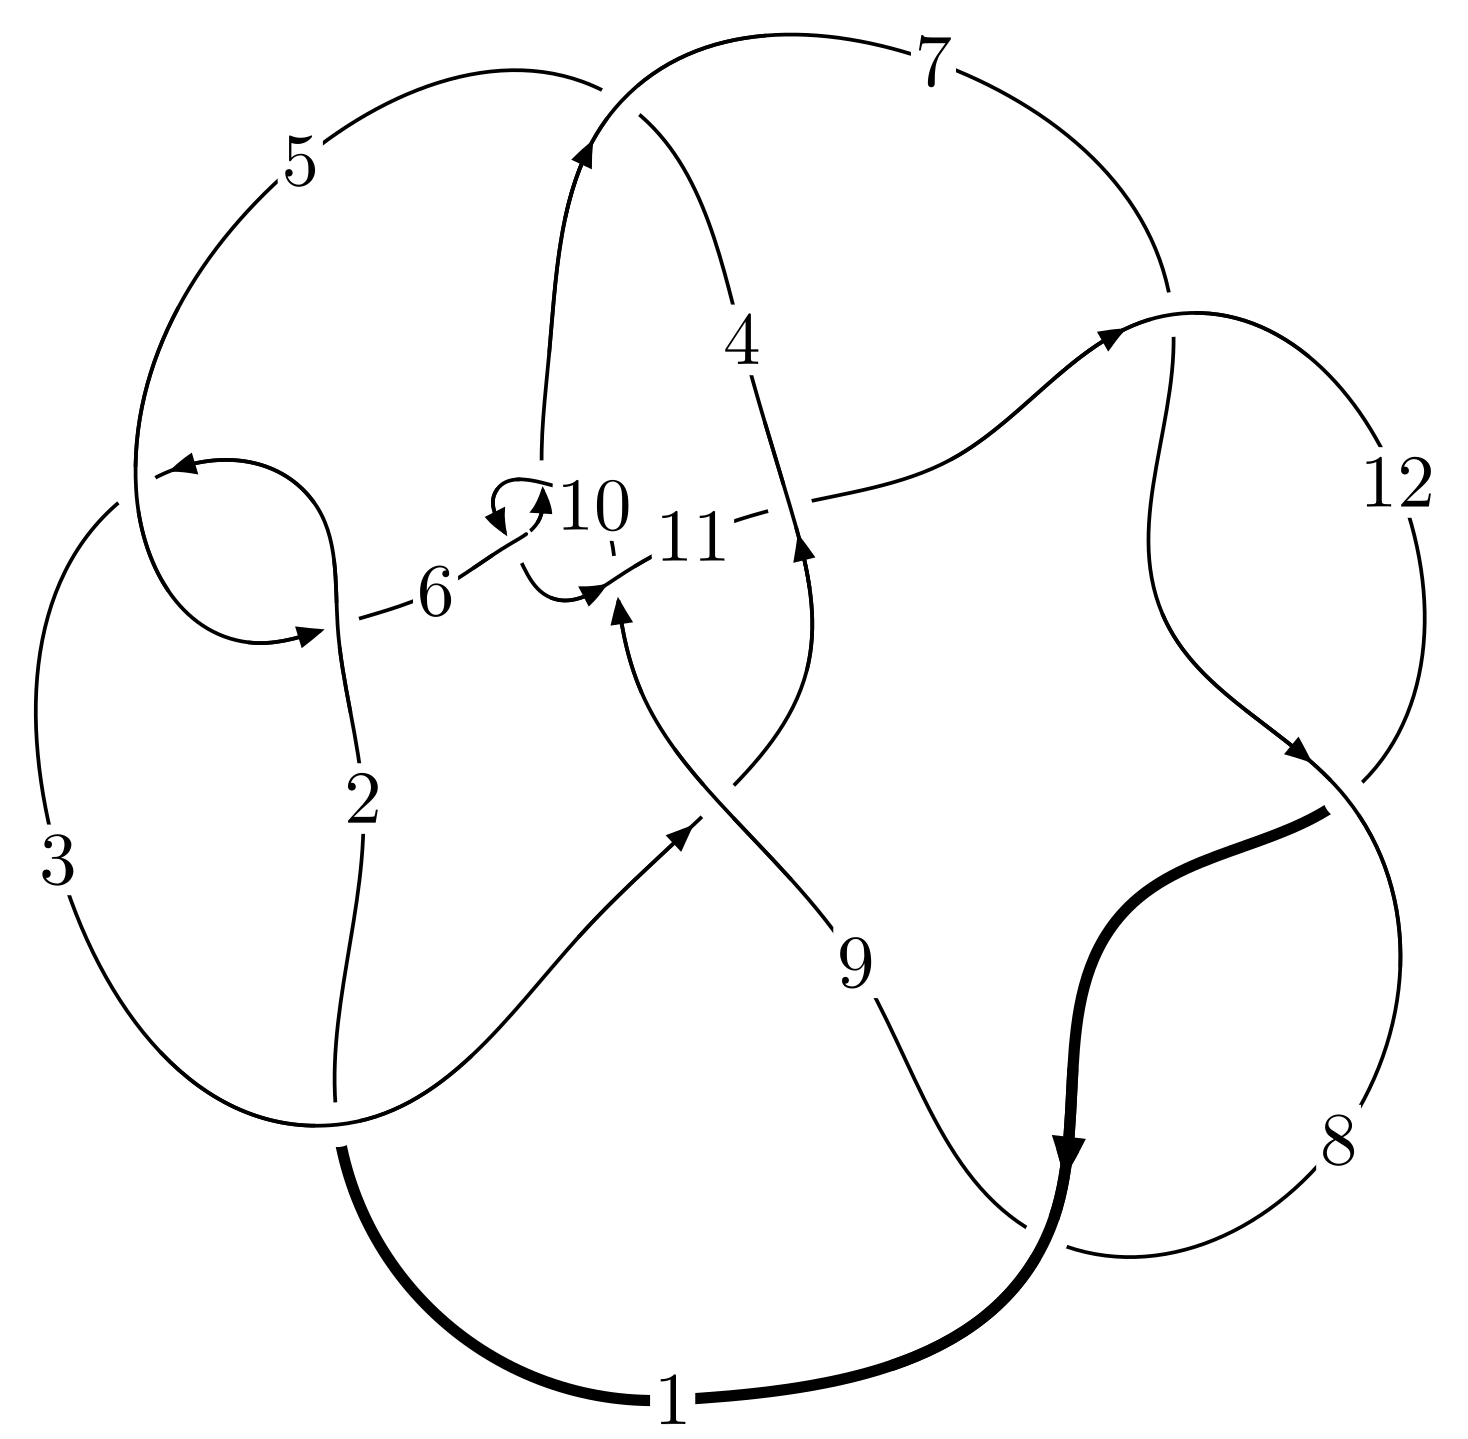
\includegraphics[width=112pt]{../../../GIT/diagram.site/Diagrams/png/987_12a_0186.png}\\
\ \ \ A knot diagram\footnotemark}&
\allowdisplaybreaks
\textbf{Linearized knot diagam} \\
\cline{2-2}
 &
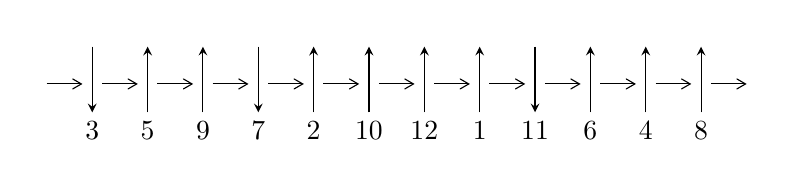
\begin{tikzpicture}[x=20pt, y=17pt]
	% nodes
	\node (C0) at (0, 0) {};
	\node (C1) at (1, 0) {};
	\node (C1U) at (1, +1) {};
	\node (C1D) at (1, -1) {3};

	\node (C2) at (2, 0) {};
	\node (C2U) at (2, +1) {};
	\node (C2D) at (2, -1) {5};

	\node (C3) at (3, 0) {};
	\node (C3U) at (3, +1) {};
	\node (C3D) at (3, -1) {9};

	\node (C4) at (4, 0) {};
	\node (C4U) at (4, +1) {};
	\node (C4D) at (4, -1) {7};

	\node (C5) at (5, 0) {};
	\node (C5U) at (5, +1) {};
	\node (C5D) at (5, -1) {2};

	\node (C6) at (6, 0) {};
	\node (C6U) at (6, +1) {};
	\node (C6D) at (6, -1) {10};

	\node (C7) at (7, 0) {};
	\node (C7U) at (7, +1) {};
	\node (C7D) at (7, -1) {12};

	\node (C8) at (8, 0) {};
	\node (C8U) at (8, +1) {};
	\node (C8D) at (8, -1) {1};

	\node (C9) at (9, 0) {};
	\node (C9U) at (9, +1) {};
	\node (C9D) at (9, -1) {11};

	\node (C10) at (10, 0) {};
	\node (C10U) at (10, +1) {};
	\node (C10D) at (10, -1) {6};

	\node (C11) at (11, 0) {};
	\node (C11U) at (11, +1) {};
	\node (C11D) at (11, -1) {4};

	\node (C12) at (12, 0) {};
	\node (C12U) at (12, +1) {};
	\node (C12D) at (12, -1) {8};
	\node (C13) at (13, 0) {};

	% arrows
	\draw[->,>={angle 60}]
	(C0) edge (C1) (C1) edge (C2) (C2) edge (C3) (C3) edge (C4) (C4) edge (C5) (C5) edge (C6) (C6) edge (C7) (C7) edge (C8) (C8) edge (C9) (C9) edge (C10) (C10) edge (C11) (C11) edge (C12) (C12) edge (C13) ;	\draw[->,>=stealth]
	(C1U) edge (C1D) (C2D) edge (C2U) (C3D) edge (C3U) (C4U) edge (C4D) (C5D) edge (C5U) (C6D) edge (C6U) (C7D) edge (C7U) (C8D) edge (C8U) (C9U) edge (C9D) (C10D) edge (C10U) (C11D) edge (C11U) (C12D) edge (C12U) ;
	\end{tikzpicture} \\
\hhline{~~} \\& 
\textbf{Solving Sequence} \\ \cline{2-2} 
 &
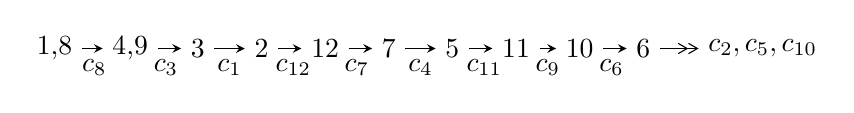
\begin{tikzpicture}[x=23pt, y=7pt]
	% node
	\node (A0) at (-1/8, 0) {1,8};
	\node (A1) at (17/16, 0) {4,9};
	\node (A2) at (17/8, 0) {3};
	\node (A3) at (25/8, 0) {2};
	\node (A4) at (33/8, 0) {12};
	\node (A5) at (41/8, 0) {7};
	\node (A6) at (49/8, 0) {5};
	\node (A7) at (57/8, 0) {11};
	\node (A8) at (65/8, 0) {10};
	\node (A9) at (73/8, 0) {6};
	\node (C1) at (1/2, -1) {$c_{8}$};
	\node (C2) at (13/8, -1) {$c_{3}$};
	\node (C3) at (21/8, -1) {$c_{1}$};
	\node (C4) at (29/8, -1) {$c_{12}$};
	\node (C5) at (37/8, -1) {$c_{7}$};
	\node (C6) at (45/8, -1) {$c_{4}$};
	\node (C7) at (53/8, -1) {$c_{11}$};
	\node (C8) at (61/8, -1) {$c_{9}$};
	\node (C9) at (69/8, -1) {$c_{6}$};
	\node (A10) at (11, 0) {$c_{2},c_{5},c_{10}$};

	% edge
	\draw[->,>=stealth]	
	(A0) edge (A1) (A1) edge (A2) (A2) edge (A3) (A3) edge (A4) (A4) edge (A5) (A5) edge (A6) (A6) edge (A7) (A7) edge (A8) (A8) edge (A9) ;
	\draw[->>,>={angle 60}]	
	(A9) edge (A10);
\end{tikzpicture} \\ 

\end{tabular} \\

\footnotetext{
The image of knot diagram is generated by the software ``\textbf{Draw programme}" developed by Andrew Bartholomew(\url{http://www.layer8.co.uk/maths/draw/index.htm\#Running-draw}), where we modified some parts for our purpose(\url{https://github.com/CATsTAILs/LinksPainter}).
}\phantom \\ \newline 
\centering \textbf{Ideals for irreducible components\footnotemark of $X_{\text{par}}$} 
 
\begin{align*}
I^u_{1}&=\langle 
-7.83274\times10^{205} u^{101}+3.91863\times10^{206} u^{100}+\cdots+3.50853\times10^{206} b+1.57493\times10^{206},\\
\phantom{I^u_{1}}&\phantom{= \langle  }1.45541\times10^{206} u^{101}-5.81604\times10^{206} u^{100}+\cdots+3.50853\times10^{206} a-4.94259\times10^{206},\\
\phantom{I^u_{1}}&\phantom{= \langle  }u^{102}-3 u^{101}+\cdots+8 u^2-1\rangle \\
I^u_{2}&=\langle 
b+a,\;-21 u^2 a+49 a^2+35 a u+10 u^2-7 a-19 u+22,\;u^3- u^2+1\rangle \\
\\
\end{align*}
\raggedright * 2 irreducible components of $\dim_{\mathbb{C}}=0$, with total 108 representations.\\
\footnotetext{All coefficients of polynomials are rational numbers. But the coefficients are sometimes approximated in decimal forms when there is not enough margin.}
\newpage
\renewcommand{\arraystretch}{1}
\centering \section*{I. $I^u_{1}= \langle -7.83\times10^{205} u^{101}+3.92\times10^{206} u^{100}+\cdots+3.51\times10^{206} b+1.57\times10^{206},\;1.46\times10^{206} u^{101}-5.82\times10^{206} u^{100}+\cdots+3.51\times10^{206} a-4.94\times10^{206},\;u^{102}-3 u^{101}+\cdots+8 u^2-1 \rangle$}
\flushleft \textbf{(i) Arc colorings}\\
\begin{tabular}{m{7pt} m{180pt} m{7pt} m{180pt} }
\flushright $a_{1}=$&$\begin{pmatrix}0\\u\end{pmatrix}$ \\
\flushright $a_{8}=$&$\begin{pmatrix}1\\0\end{pmatrix}$ \\
\flushright $a_{4}=$&$\begin{pmatrix}-0.414820 u^{101}+1.65768 u^{100}+\cdots-2.81202 u+1.40873\\0.223249 u^{101}-1.11689 u^{100}+\cdots+4.14860 u-0.448887\end{pmatrix}$ \\
\flushright $a_{9}=$&$\begin{pmatrix}1\\- u^2\end{pmatrix}$ \\
\flushright $a_{3}=$&$\begin{pmatrix}-0.476650 u^{101}+1.78872 u^{100}+\cdots-6.54580 u+1.44440\\-0.106382 u^{101}+0.250932 u^{100}+\cdots+4.21043 u-0.394429\end{pmatrix}$ \\
\flushright $a_{2}=$&$\begin{pmatrix}0.643889 u^{101}-1.30576 u^{100}+\cdots+0.763924 u+0.781537\\-1.78169 u^{101}+3.56162 u^{100}+\cdots+1.44173 u-1.38730\end{pmatrix}$ \\
\flushright $a_{12}=$&$\begin{pmatrix}- u\\u\end{pmatrix}$ \\
\flushright $a_{7}=$&$\begin{pmatrix}- u^2+1\\u^2\end{pmatrix}$ \\
\flushright $a_{5}=$&$\begin{pmatrix}-0.498144 u^{101}+1.88558 u^{100}+\cdots-6.66075 u+1.65027\\-0.184868 u^{101}+0.302979 u^{100}+\cdots+3.65716 u-0.275453\end{pmatrix}$ \\
\flushright $a_{11}=$&$\begin{pmatrix}0.649518 u^{101}-1.16680 u^{100}+\cdots+1.05959 u-0.0364924\\-0.379081 u^{101}+0.596176 u^{100}+\cdots-0.990884 u-0.301947\end{pmatrix}$ \\
\flushright $a_{10}=$&$\begin{pmatrix}-1.00635 u^{101}+1.44490 u^{100}+\cdots-0.159676 u+0.574120\\1.43698 u^{101}-2.29172 u^{100}+\cdots+0.720833 u+0.738916\end{pmatrix}$ \\
\flushright $a_{6}=$&$\begin{pmatrix}-0.270437 u^{101}+0.570627 u^{100}+\cdots-0.0687015 u+0.338440\\-0.379081 u^{101}+0.596176 u^{100}+\cdots-0.990884 u-0.301947\end{pmatrix}$\\&\end{tabular}
\flushleft \textbf{(ii) Obstruction class $= -1$}\\~\\
\flushleft \textbf{(iii) Cusp Shapes $= -1.59541 u^{101}+0.803708 u^{100}+\cdots+5.97952 u+6.60121$}\\~\\
\newpage\renewcommand{\arraystretch}{1}
\flushleft \textbf{(iv) u-Polynomials at the component}\newline \\
\begin{tabular}{m{50pt}|m{274pt}}
Crossings & \hspace{64pt}u-Polynomials at each crossing \\
\hline $$\begin{aligned}c_{1}\end{aligned}$$&$\begin{aligned}
&u^{102}+36 u^{101}+\cdots-20973 u+2401
\end{aligned}$\\
\hline $$\begin{aligned}c_{2},c_{5}\end{aligned}$$&$\begin{aligned}
&u^{102}+4 u^{101}+\cdots-197 u+49
\end{aligned}$\\
\hline $$\begin{aligned}c_{3}\end{aligned}$$&$\begin{aligned}
&49(49 u^{102}-70 u^{101}+\cdots-5.45423\times10^{8} u-2.55402\times10^{8})
\end{aligned}$\\
\hline $$\begin{aligned}c_{4}\end{aligned}$$&$\begin{aligned}
&49(49 u^{102}-126 u^{101}+\cdots+2407086 u+356047)
\end{aligned}$\\
\hline $$\begin{aligned}c_{6},c_{10}\end{aligned}$$&$\begin{aligned}
&u^{102}-3 u^{101}+\cdots+6 u-1
\end{aligned}$\\
\hline $$\begin{aligned}c_{7},c_{8},c_{12}\end{aligned}$$&$\begin{aligned}
&u^{102}-3 u^{101}+\cdots+8 u^2-1
\end{aligned}$\\
\hline $$\begin{aligned}c_{9}\end{aligned}$$&$\begin{aligned}
&u^{102}+43 u^{101}+\cdots-16 u+1
\end{aligned}$\\
\hline $$\begin{aligned}c_{11}\end{aligned}$$&$\begin{aligned}
&u^{102}-5 u^{101}+\cdots+174048 u-21952
\end{aligned}$\\
\hline
\end{tabular}\\~\\
\newpage\renewcommand{\arraystretch}{1}
\flushleft \textbf{(v) Riley Polynomials at the component}\newline \\
\begin{tabular}{m{50pt}|m{274pt}}
Crossings & \hspace{64pt}Riley Polynomials at each crossing \\
\hline $$\begin{aligned}c_{1}\end{aligned}$$&$\begin{aligned}
&y^{102}+64 y^{101}+\cdots-2635965389 y+5764801
\end{aligned}$\\
\hline $$\begin{aligned}c_{2},c_{5}\end{aligned}$$&$\begin{aligned}
&y^{102}+36 y^{101}+\cdots-20973 y+2401
\end{aligned}$\\
\hline $$\begin{aligned}c_{3}\end{aligned}$$&$\begin{aligned}
&2401(2401 y^{102}-211092 y^{101}+\cdots-1.97644\times10^{18} y+6.52300\times10^{16})
\end{aligned}$\\
\hline $$\begin{aligned}c_{4}\end{aligned}$$&$\begin{aligned}
&2401\\
&\cdot(2401 y^{102}+47530 y^{101}+\cdots-8262494848850 y+126769466209)
\end{aligned}$\\
\hline $$\begin{aligned}c_{6},c_{10}\end{aligned}$$&$\begin{aligned}
&y^{102}+43 y^{101}+\cdots-16 y+1
\end{aligned}$\\
\hline $$\begin{aligned}c_{7},c_{8},c_{12}\end{aligned}$$&$\begin{aligned}
&y^{102}-101 y^{101}+\cdots-16 y+1
\end{aligned}$\\
\hline $$\begin{aligned}c_{9}\end{aligned}$$&$\begin{aligned}
&y^{102}+35 y^{101}+\cdots+372 y+1
\end{aligned}$\\
\hline $$\begin{aligned}c_{11}\end{aligned}$$&$\begin{aligned}
&y^{102}-35 y^{101}+\cdots-8007738368 y+481890304
\end{aligned}$\\
\hline
\end{tabular}\\~\\
\newpage\flushleft \textbf{(vi) Complex Volumes and Cusp Shapes}
$$\begin{array}{c|c|c}  
\text{Solutions to }I^u_{1}& \I (\text{vol} + \sqrt{-1}CS) & \text{Cusp shape}\\
 \hline 
\begin{aligned}
u &= \phantom{-}0.463265 + 0.883839 I \\
a &= \phantom{-}0.035861 + 0.629190 I \\
b &= -0.374833 + 0.308984 I\end{aligned}
 & \phantom{-}4.20876 + 2.87950 I & \phantom{-0.000000 } 0 \\ \hline\begin{aligned}
u &= \phantom{-}0.463265 - 0.883839 I \\
a &= \phantom{-}0.035861 - 0.629190 I \\
b &= -0.374833 - 0.308984 I\end{aligned}
 & \phantom{-}4.20876 - 2.87950 I & \phantom{-0.000000 } 0 \\ \hline\begin{aligned}
u &= -0.577868 + 0.813521 I \\
a &= \phantom{-}0.472549 + 0.598092 I \\
b &= \phantom{-}0.909310 - 0.193187 I\end{aligned}
 & \phantom{-}1.8572 - 14.1354 I & \phantom{-0.000000 } 0 \\ \hline\begin{aligned}
u &= -0.577868 - 0.813521 I \\
a &= \phantom{-}0.472549 - 0.598092 I \\
b &= \phantom{-}0.909310 + 0.193187 I\end{aligned}
 & \phantom{-}1.8572 + 14.1354 I & \phantom{-0.000000 } 0 \\ \hline\begin{aligned}
u &= \phantom{-}0.954849 + 0.281344 I \\
a &= -0.041980 - 0.257493 I \\
b &= \phantom{-}0.307337 - 0.426122 I\end{aligned}
 & \phantom{-}0.469698 + 0.856662 I & \phantom{-0.000000 } 0 \\ \hline\begin{aligned}
u &= \phantom{-}0.954849 - 0.281344 I \\
a &= -0.041980 + 0.257493 I \\
b &= \phantom{-}0.307337 + 0.426122 I\end{aligned}
 & \phantom{-}0.469698 - 0.856662 I & \phantom{-0.000000 } 0 \\ \hline\begin{aligned}
u &= \phantom{-}0.570625 + 0.835524 I \\
a &= -0.368172 + 0.608065 I \\
b &= -0.798500 - 0.073995 I\end{aligned}
 & \phantom{-}3.77268 + 8.13531 I & \phantom{-0.000000 } 0 \\ \hline\begin{aligned}
u &= \phantom{-}0.570625 - 0.835524 I \\
a &= -0.368172 - 0.608065 I \\
b &= -0.798500 + 0.073995 I\end{aligned}
 & \phantom{-}3.77268 - 8.13531 I & \phantom{-0.000000 } 0 \\ \hline\begin{aligned}
u &= \phantom{-}0.645597 + 0.723769 I \\
a &= \phantom{-}0.473710 - 0.425187 I \\
b &= \phantom{-}0.771863 - 0.005327 I\end{aligned}
 & \phantom{-}4.91261 + 2.43397 I & \phantom{-0.000000 } 0 \\ \hline\begin{aligned}
u &= \phantom{-}0.645597 - 0.723769 I \\
a &= \phantom{-}0.473710 + 0.425187 I \\
b &= \phantom{-}0.771863 + 0.005327 I\end{aligned}
 & \phantom{-}4.91261 - 2.43397 I & \phantom{-0.000000 } 0\\
 \hline 
 \end{array}$$\newpage$$\begin{array}{c|c|c}  
\text{Solutions to }I^u_{1}& \I (\text{vol} + \sqrt{-1}CS) & \text{Cusp shape}\\
 \hline 
\begin{aligned}
u &= -0.573506 + 0.862250 I \\
a &= \phantom{-}0.260008 - 0.666688 I \\
b &= -0.325821 - 0.399726 I\end{aligned}
 & \phantom{-}1.77977 + 8.59624 I & \phantom{-0.000000 } 0 \\ \hline\begin{aligned}
u &= -0.573506 - 0.862250 I \\
a &= \phantom{-}0.260008 + 0.666688 I \\
b &= -0.325821 + 0.399726 I\end{aligned}
 & \phantom{-}1.77977 - 8.59624 I & \phantom{-0.000000 } 0 \\ \hline\begin{aligned}
u &= \phantom{-}0.625060 + 0.855119 I \\
a &= -0.072253 - 0.595095 I \\
b &= \phantom{-}0.424918 - 0.290495 I\end{aligned}
 & \phantom{-}3.86224 - 2.49227 I & \phantom{-0.000000 } 0 \\ \hline\begin{aligned}
u &= \phantom{-}0.625060 - 0.855119 I \\
a &= -0.072253 + 0.595095 I \\
b &= \phantom{-}0.424918 + 0.290495 I\end{aligned}
 & \phantom{-}3.86224 + 2.49227 I & \phantom{-0.000000 } 0 \\ \hline\begin{aligned}
u &= -0.620905 + 0.706635 I \\
a &= -0.630977 - 0.363939 I \\
b &= -0.865313 + 0.085922 I\end{aligned}
 & \phantom{-}3.41050 - 8.30399 I & \phantom{-0.000000 } 0 \\ \hline\begin{aligned}
u &= -0.620905 - 0.706635 I \\
a &= -0.630977 + 0.363939 I \\
b &= -0.865313 - 0.085922 I\end{aligned}
 & \phantom{-}3.41050 + 8.30399 I & \phantom{-0.000000 } 0 \\ \hline\begin{aligned}
u &= -0.413392 + 0.842069 I \\
a &= -0.198359 + 0.651935 I \\
b &= \phantom{-}0.204367 + 0.456259 I\end{aligned}
 & \phantom{-}2.71161 + 3.24755 I & \phantom{-0.000000 } 0 \\ \hline\begin{aligned}
u &= -0.413392 - 0.842069 I \\
a &= -0.198359 - 0.651935 I \\
b &= \phantom{-}0.204367 - 0.456259 I\end{aligned}
 & \phantom{-}2.71161 - 3.24755 I & \phantom{-0.000000 } 0 \\ \hline\begin{aligned}
u &= -0.636919 + 0.931863 I \\
a &= \phantom{-}0.212442 + 0.374659 I \\
b &= \phantom{-}0.398835 - 0.155929 I\end{aligned}
 & -3.21005 - 5.48312 I & \phantom{-0.000000 } 0 \\ \hline\begin{aligned}
u &= -0.636919 - 0.931863 I \\
a &= \phantom{-}0.212442 - 0.374659 I \\
b &= \phantom{-}0.398835 + 0.155929 I\end{aligned}
 & -3.21005 + 5.48312 I & \phantom{-0.000000 } 0\\
 \hline 
 \end{array}$$\newpage$$\begin{array}{c|c|c}  
\text{Solutions to }I^u_{1}& \I (\text{vol} + \sqrt{-1}CS) & \text{Cusp shape}\\
 \hline 
\begin{aligned}
u &= -1.007680 + 0.591458 I \\
a &= \phantom{-}0.183227 - 0.022455 I \\
b &= -0.112994 - 0.513226 I\end{aligned}
 & -3.52837 - 4.73810 I & \phantom{-0.000000 } 0 \\ \hline\begin{aligned}
u &= -1.007680 - 0.591458 I \\
a &= \phantom{-}0.183227 + 0.022455 I \\
b &= -0.112994 + 0.513226 I\end{aligned}
 & -3.52837 + 4.73810 I & \phantom{-0.000000 } 0 \\ \hline\begin{aligned}
u &= -0.683434 + 0.363431 I \\
a &= \phantom{-}0.298305 - 0.422340 I \\
b &= -0.606073 - 0.754369 I\end{aligned}
 & -2.25139 + 3.24449 I & \phantom{-0.000000 } 0 \\ \hline\begin{aligned}
u &= -0.683434 - 0.363431 I \\
a &= \phantom{-}0.298305 + 0.422340 I \\
b &= -0.606073 + 0.754369 I\end{aligned}
 & -2.25139 - 3.24449 I & \phantom{-0.000000 } 0 \\ \hline\begin{aligned}
u &= -0.850848 + 0.891750 I \\
a &= -0.009513 - 0.251567 I \\
b &= -0.350113 + 0.018910 I\end{aligned}
 & -2.71812 - 0.96266 I & \phantom{-0.000000 } 0 \\ \hline\begin{aligned}
u &= -0.850848 - 0.891750 I \\
a &= -0.009513 + 0.251567 I \\
b &= -0.350113 - 0.018910 I\end{aligned}
 & -2.71812 + 0.96266 I & \phantom{-0.000000 } 0 \\ \hline\begin{aligned}
u &= -0.248176 + 0.709636 I \\
a &= \phantom{-}0.975285 + 0.448105 I \\
b &= \phantom{-}0.373511 - 0.188307 I\end{aligned}
 & -5.59230 + 0.19794 I & \phantom{-0.000000 } 0 \\ \hline\begin{aligned}
u &= -0.248176 - 0.709636 I \\
a &= \phantom{-}0.975285 - 0.448105 I \\
b &= \phantom{-}0.373511 + 0.188307 I\end{aligned}
 & -5.59230 - 0.19794 I & \phantom{-0.000000 } 0 \\ \hline\begin{aligned}
u &= -0.531434 + 0.485622 I \\
a &= -0.403276 + 0.205773 I \\
b &= -0.499838 + 0.308340 I\end{aligned}
 & -2.05892 - 1.75560 I & \phantom{-}2.99481 + 4.92518 I \\ \hline\begin{aligned}
u &= -0.531434 - 0.485622 I \\
a &= -0.403276 - 0.205773 I \\
b &= -0.499838 - 0.308340 I\end{aligned}
 & -2.05892 + 1.75560 I & \phantom{-}2.99481 - 4.92518 I\\
 \hline 
 \end{array}$$\newpage$$\begin{array}{c|c|c}  
\text{Solutions to }I^u_{1}& \I (\text{vol} + \sqrt{-1}CS) & \text{Cusp shape}\\
 \hline 
\begin{aligned}
u &= \phantom{-}1.302550 + 0.030953 I \\
a &= -0.09799 + 1.82910 I \\
b &= \phantom{-}0.52176 - 1.51246 I\end{aligned}
 & \phantom{-}4.38155 - 0.95243 I & \phantom{-0.000000 } 0 \\ \hline\begin{aligned}
u &= \phantom{-}1.302550 - 0.030953 I \\
a &= -0.09799 - 1.82910 I \\
b &= \phantom{-}0.52176 + 1.51246 I\end{aligned}
 & \phantom{-}4.38155 + 0.95243 I & \phantom{-0.000000 } 0 \\ \hline\begin{aligned}
u &= -0.331178 + 0.573078 I \\
a &= \phantom{-}1.49364 + 1.09467 I \\
b &= \phantom{-}0.537434 - 0.209557 I\end{aligned}
 & -3.34096 - 6.68172 I & \phantom{-}1.38828 + 9.11332 I \\ \hline\begin{aligned}
u &= -0.331178 - 0.573078 I \\
a &= \phantom{-}1.49364 - 1.09467 I \\
b &= \phantom{-}0.537434 + 0.209557 I\end{aligned}
 & -3.34096 + 6.68172 I & \phantom{-}1.38828 - 9.11332 I \\ \hline\begin{aligned}
u &= -1.356920 + 0.044854 I \\
a &= \phantom{-}1.93962 + 2.56034 I \\
b &= -2.34234 - 2.36543 I\end{aligned}
 & \phantom{-}4.60358 - 3.83826 I & \phantom{-0.000000 } 0 \\ \hline\begin{aligned}
u &= -1.356920 - 0.044854 I \\
a &= \phantom{-}1.93962 - 2.56034 I \\
b &= -2.34234 + 2.36543 I\end{aligned}
 & \phantom{-}4.60358 + 3.83826 I & \phantom{-0.000000 } 0 \\ \hline\begin{aligned}
u &= \phantom{-}1.392320 + 0.193973 I \\
a &= -1.361140 - 0.145231 I \\
b &= \phantom{-}2.13438 + 0.72591 I\end{aligned}
 & -0.40709 + 2.94965 I & \phantom{-0.000000 } 0 \\ \hline\begin{aligned}
u &= \phantom{-}1.392320 - 0.193973 I \\
a &= -1.361140 + 0.145231 I \\
b &= \phantom{-}2.13438 - 0.72591 I\end{aligned}
 & -0.40709 - 2.94965 I & \phantom{-0.000000 } 0 \\ \hline\begin{aligned}
u &= \phantom{-}0.238337 + 0.527550 I \\
a &= -0.88698 + 1.20969 I \\
b &= -0.554896 - 0.179442 I\end{aligned}
 & -1.56944 + 2.20050 I & \phantom{-}3.50144 - 4.94016 I \\ \hline\begin{aligned}
u &= \phantom{-}0.238337 - 0.527550 I \\
a &= -0.88698 - 1.20969 I \\
b &= -0.554896 + 0.179442 I\end{aligned}
 & -1.56944 - 2.20050 I & \phantom{-}3.50144 + 4.94016 I\\
 \hline 
 \end{array}$$\newpage$$\begin{array}{c|c|c}  
\text{Solutions to }I^u_{1}& \I (\text{vol} + \sqrt{-1}CS) & \text{Cusp shape}\\
 \hline 
\begin{aligned}
u &= -1.43398 + 0.08205 I \\
a &= \phantom{-}2.14168 - 0.02876 I \\
b &= -2.86553 - 0.26922 I\end{aligned}
 & \phantom{-}4.10044 - 3.96620 I & \phantom{-0.000000 } 0 \\ \hline\begin{aligned}
u &= -1.43398 - 0.08205 I \\
a &= \phantom{-}2.14168 + 0.02876 I \\
b &= -2.86553 + 0.26922 I\end{aligned}
 & \phantom{-}4.10044 + 3.96620 I & \phantom{-0.000000 } 0 \\ \hline\begin{aligned}
u &= -1.43341 + 0.13902 I \\
a &= \phantom{-}2.02100 + 0.05752 I \\
b &= -3.17918 + 0.14402 I\end{aligned}
 & \phantom{-}3.87436 - 4.46338 I & \phantom{-0.000000 } 0 \\ \hline\begin{aligned}
u &= -1.43341 - 0.13902 I \\
a &= \phantom{-}2.02100 - 0.05752 I \\
b &= -3.17918 - 0.14402 I\end{aligned}
 & \phantom{-}3.87436 + 4.46338 I & \phantom{-0.000000 } 0 \\ \hline\begin{aligned}
u &= \phantom{-}0.555079 + 0.064471 I \\
a &= \phantom{-}2.01633 + 1.39157 I \\
b &= \phantom{-}0.267624 - 0.229465 I\end{aligned}
 & \phantom{-}3.09413 - 0.79742 I & \phantom{-}15.9448 + 0.0041 I \\ \hline\begin{aligned}
u &= \phantom{-}0.555079 - 0.064471 I \\
a &= \phantom{-}2.01633 - 1.39157 I \\
b &= \phantom{-}0.267624 + 0.229465 I\end{aligned}
 & \phantom{-}3.09413 + 0.79742 I & \phantom{-}15.9448 - 0.0041 I \\ \hline\begin{aligned}
u &= -0.542802 + 0.100561 I \\
a &= -1.78669 + 2.04178 I \\
b &= -0.291885 - 0.324437 I\end{aligned}
 & \phantom{-}2.93517 - 4.09723 I & \phantom{-}15.0428 + 7.4403 I \\ \hline\begin{aligned}
u &= -0.542802 - 0.100561 I \\
a &= -1.78669 - 2.04178 I \\
b &= -0.291885 + 0.324437 I\end{aligned}
 & \phantom{-}2.93517 + 4.09723 I & \phantom{-}15.0428 - 7.4403 I \\ \hline\begin{aligned}
u &= -1.45457 + 0.00026 I \\
a &= -3.91802 + 2.34344 I \\
b &= \phantom{-}4.10714 - 2.07963 I\end{aligned}
 & \phantom{-}5.01824 - 0.26285 I & \phantom{-0.000000 } 0 \\ \hline\begin{aligned}
u &= -1.45457 - 0.00026 I \\
a &= -3.91802 - 2.34344 I \\
b &= \phantom{-}4.10714 + 2.07963 I\end{aligned}
 & \phantom{-}5.01824 + 0.26285 I & \phantom{-0.000000 } 0\\
 \hline 
 \end{array}$$\newpage$$\begin{array}{c|c|c}  
\text{Solutions to }I^u_{1}& \I (\text{vol} + \sqrt{-1}CS) & \text{Cusp shape}\\
 \hline 
\begin{aligned}
u &= \phantom{-}1.44682 + 0.16164 I \\
a &= -2.08341 - 0.23008 I \\
b &= \phantom{-}3.41637 + 0.72748 I\end{aligned}
 & \phantom{-}2.41336 + 9.25279 I & \phantom{-0.000000 } 0 \\ \hline\begin{aligned}
u &= \phantom{-}1.44682 - 0.16164 I \\
a &= -2.08341 + 0.23008 I \\
b &= \phantom{-}3.41637 - 0.72748 I\end{aligned}
 & \phantom{-}2.41336 - 9.25279 I & \phantom{-0.000000 } 0 \\ \hline\begin{aligned}
u &= \phantom{-}0.438840 + 0.304153 I \\
a &= -0.37871 + 3.16877 I \\
b &= \phantom{-}0.000805 - 0.274983 I\end{aligned}
 & \phantom{-}0.99489 + 6.60455 I & \phantom{-}9.1908 - 11.8145 I \\ \hline\begin{aligned}
u &= \phantom{-}0.438840 - 0.304153 I \\
a &= -0.37871 - 3.16877 I \\
b &= \phantom{-}0.000805 + 0.274983 I\end{aligned}
 & \phantom{-}0.99489 - 6.60455 I & \phantom{-}9.1908 + 11.8145 I \\ \hline\begin{aligned}
u &= \phantom{-}1.47118 + 0.03655 I \\
a &= \phantom{-}0.225848 - 0.757857 I \\
b &= -0.254049 + 0.004641 I\end{aligned}
 & \phantom{-}6.45968 + 2.80804 I & \phantom{-0.000000 } 0 \\ \hline\begin{aligned}
u &= \phantom{-}1.47118 - 0.03655 I \\
a &= \phantom{-}0.225848 + 0.757857 I \\
b &= -0.254049 - 0.004641 I\end{aligned}
 & \phantom{-}6.45968 - 2.80804 I & \phantom{-0.000000 } 0 \\ \hline\begin{aligned}
u &= -0.445734 + 0.249585 I \\
a &= -0.09740 + 3.08006 I \\
b &= -0.118542 - 0.379389 I\end{aligned}
 & \phantom{-}1.62557 - 1.89948 I & \phantom{-}11.64063 + 5.47837 I \\ \hline\begin{aligned}
u &= -0.445734 - 0.249585 I \\
a &= -0.09740 - 3.08006 I \\
b &= -0.118542 + 0.379389 I\end{aligned}
 & \phantom{-}1.62557 + 1.89948 I & \phantom{-}11.64063 - 5.47837 I \\ \hline\begin{aligned}
u &= \phantom{-}1.49066 + 0.00722 I \\
a &= \phantom{-}1.95997 + 0.26537 I \\
b &= -2.32422 - 0.51113 I\end{aligned}
 & \phantom{-}4.98713 + 2.80685 I & \phantom{-0.000000 } 0 \\ \hline\begin{aligned}
u &= \phantom{-}1.49066 - 0.00722 I \\
a &= \phantom{-}1.95997 - 0.26537 I \\
b &= -2.32422 + 0.51113 I\end{aligned}
 & \phantom{-}4.98713 - 2.80685 I & \phantom{-0.000000 } 0\\
 \hline 
 \end{array}$$\newpage$$\begin{array}{c|c|c}  
\text{Solutions to }I^u_{1}& \I (\text{vol} + \sqrt{-1}CS) & \text{Cusp shape}\\
 \hline 
\begin{aligned}
u &= -1.48883 + 0.07877 I \\
a &= \phantom{-}1.23379 + 0.94819 I \\
b &= -2.17835 - 2.35342 I\end{aligned}
 & \phantom{-}7.34892 - 7.92883 I & \phantom{-0.000000 } 0 \\ \hline\begin{aligned}
u &= -1.48883 - 0.07877 I \\
a &= \phantom{-}1.23379 - 0.94819 I \\
b &= -2.17835 + 2.35342 I\end{aligned}
 & \phantom{-}7.34892 + 7.92883 I & \phantom{-0.000000 } 0 \\ \hline\begin{aligned}
u &= \phantom{-}1.49016 + 0.06629 I \\
a &= -0.695866 + 0.847577 I \\
b &= \phantom{-}1.22694 - 2.31857 I\end{aligned}
 & \phantom{-}8.00924 + 3.00206 I & \phantom{-0.000000 } 0 \\ \hline\begin{aligned}
u &= \phantom{-}1.49016 - 0.06629 I \\
a &= -0.695866 - 0.847577 I \\
b &= \phantom{-}1.22694 + 2.31857 I\end{aligned}
 & \phantom{-}8.00924 - 3.00206 I & \phantom{-0.000000 } 0 \\ \hline\begin{aligned}
u &= -1.49232\phantom{ +0.000000I} \\
a &= -1.81358\phantom{ +0.000000I} \\
b &= \phantom{-}2.56753\phantom{ +0.000000I}\end{aligned}
 & \phantom{-}7.18734\phantom{ +0.000000I} & \phantom{-0.000000 } 0 \\ \hline\begin{aligned}
u &= \phantom{-}1.50974 + 0.02638 I \\
a &= \phantom{-}1.57497 + 0.79438 I \\
b &= -2.75438 - 2.05820 I\end{aligned}
 & \phantom{-}9.69521 + 4.54334 I & \phantom{-0.000000 } 0 \\ \hline\begin{aligned}
u &= \phantom{-}1.50974 - 0.02638 I \\
a &= \phantom{-}1.57497 - 0.79438 I \\
b &= -2.75438 + 2.05820 I\end{aligned}
 & \phantom{-}9.69521 - 4.54334 I & \phantom{-0.000000 } 0 \\ \hline\begin{aligned}
u &= -1.51090 + 0.01774 I \\
a &= -1.88274 + 0.55860 I \\
b &= \phantom{-}3.30537 - 1.45935 I\end{aligned}
 & \phantom{-}9.88746 + 0.50387 I & \phantom{-0.000000 } 0 \\ \hline\begin{aligned}
u &= -1.51090 - 0.01774 I \\
a &= -1.88274 - 0.55860 I \\
b &= \phantom{-}3.30537 + 1.45935 I\end{aligned}
 & \phantom{-}9.88746 - 0.50387 I & \phantom{-0.000000 } 0 \\ \hline\begin{aligned}
u &= \phantom{-}0.283962 + 0.396183 I \\
a &= -0.64955 + 1.95378 I \\
b &= -0.490466 - 0.348361 I\end{aligned}
 & -1.42104 + 2.40116 I & \phantom{-}2.87491 - 6.25860 I\\
 \hline 
 \end{array}$$\newpage$$\begin{array}{c|c|c}  
\text{Solutions to }I^u_{1}& \I (\text{vol} + \sqrt{-1}CS) & \text{Cusp shape}\\
 \hline 
\begin{aligned}
u &= \phantom{-}0.283962 - 0.396183 I \\
a &= -0.64955 - 1.95378 I \\
b &= -0.490466 + 0.348361 I\end{aligned}
 & -1.42104 - 2.40116 I & \phantom{-}2.87491 + 6.25860 I \\ \hline\begin{aligned}
u &= \phantom{-}0.457504\phantom{ +0.000000I} \\
a &= \phantom{-}0.629904\phantom{ +0.000000I} \\
b &= \phantom{-}0.399832\phantom{ +0.000000I}\end{aligned}
 & \phantom{-}0.720872\phantom{ +0.000000I} & \phantom{-}13.9880\phantom{ +0.000000I} \\ \hline\begin{aligned}
u &= -0.016041 + 0.449349 I \\
a &= -0.033429 + 0.542654 I \\
b &= -0.287665 + 0.922896 I\end{aligned}
 & \phantom{-}0.87311 + 2.39546 I & \phantom{-}3.08710 - 3.61565 I \\ \hline\begin{aligned}
u &= -0.016041 - 0.449349 I \\
a &= -0.033429 - 0.542654 I \\
b &= -0.287665 - 0.922896 I\end{aligned}
 & \phantom{-}0.87311 - 2.39546 I & \phantom{-}3.08710 + 3.61565 I \\ \hline\begin{aligned}
u &= \phantom{-}0.392748 + 0.215550 I \\
a &= -0.469063 - 0.870049 I \\
b &= \phantom{-}1.52815 - 0.13896 I\end{aligned}
 & -0.880180 - 0.202294 I & \phantom{-}9.92790 - 3.57486 I \\ \hline\begin{aligned}
u &= \phantom{-}0.392748 - 0.215550 I \\
a &= -0.469063 + 0.870049 I \\
b &= \phantom{-}1.52815 + 0.13896 I\end{aligned}
 & -0.880180 + 0.202294 I & \phantom{-}9.92790 + 3.57486 I \\ \hline\begin{aligned}
u &= \phantom{-}1.56060 + 0.23251 I \\
a &= \phantom{-}1.87185 + 0.03629 I \\
b &= -2.88208 - 0.61189 I\end{aligned}
 & \phantom{-}10.5879 + 11.7701 I & \phantom{-0.000000 } 0 \\ \hline\begin{aligned}
u &= \phantom{-}1.56060 - 0.23251 I \\
a &= \phantom{-}1.87185 - 0.03629 I \\
b &= -2.88208 + 0.61189 I\end{aligned}
 & \phantom{-}10.5879 - 11.7701 I & \phantom{-0.000000 } 0 \\ \hline\begin{aligned}
u &= \phantom{-}1.54397 + 0.34268 I \\
a &= -0.788558 + 0.471126 I \\
b &= \phantom{-}1.46417 - 0.57180 I\end{aligned}
 & \phantom{-}9.02348 + 1.22948 I & \phantom{-0.000000 } 0 \\ \hline\begin{aligned}
u &= \phantom{-}1.54397 - 0.34268 I \\
a &= -0.788558 - 0.471126 I \\
b &= \phantom{-}1.46417 + 0.57180 I\end{aligned}
 & \phantom{-}9.02348 - 1.22948 I & \phantom{-0.000000 } 0\\
 \hline 
 \end{array}$$\newpage$$\begin{array}{c|c|c}  
\text{Solutions to }I^u_{1}& \I (\text{vol} + \sqrt{-1}CS) & \text{Cusp shape}\\
 \hline 
\begin{aligned}
u &= \phantom{-}1.55874 + 0.27948 I \\
a &= -1.91507 + 0.03940 I \\
b &= \phantom{-}2.88329 + 0.47808 I\end{aligned}
 & \phantom{-}8.8410 + 18.1545 I & \phantom{-0.000000 } 0 \\ \hline\begin{aligned}
u &= \phantom{-}1.55874 - 0.27948 I \\
a &= -1.91507 - 0.03940 I \\
b &= \phantom{-}2.88329 - 0.47808 I\end{aligned}
 & \phantom{-}8.8410 - 18.1545 I & \phantom{-0.000000 } 0 \\ \hline\begin{aligned}
u &= -1.56710 + 0.23333 I \\
a &= -1.75578 - 0.08898 I \\
b &= \phantom{-}2.74749 - 0.34774 I\end{aligned}
 & \phantom{-}12.19110 - 5.95346 I & \phantom{-0.000000 } 0 \\ \hline\begin{aligned}
u &= -1.56710 - 0.23333 I \\
a &= -1.75578 + 0.08898 I \\
b &= \phantom{-}2.74749 + 0.34774 I\end{aligned}
 & \phantom{-}12.19110 + 5.95346 I & \phantom{-0.000000 } 0 \\ \hline\begin{aligned}
u &= -1.55962 + 0.28624 I \\
a &= \phantom{-}1.75143 + 0.15406 I \\
b &= -2.70324 + 0.25575 I\end{aligned}
 & \phantom{-}10.7337 - 12.2501 I & \phantom{-0.000000 } 0 \\ \hline\begin{aligned}
u &= -1.55962 - 0.28624 I \\
a &= \phantom{-}1.75143 - 0.15406 I \\
b &= -2.70324 - 0.25575 I\end{aligned}
 & \phantom{-}10.7337 + 12.2501 I & \phantom{-0.000000 } 0 \\ \hline\begin{aligned}
u &= -1.55677 + 0.31983 I \\
a &= \phantom{-}1.101370 + 0.405380 I \\
b &= -1.88769 - 0.35195 I\end{aligned}
 & \phantom{-}10.82960 - 7.34873 I & \phantom{-0.000000 } 0 \\ \hline\begin{aligned}
u &= -1.55677 - 0.31983 I \\
a &= \phantom{-}1.101370 - 0.405380 I \\
b &= -1.88769 + 0.35195 I\end{aligned}
 & \phantom{-}10.82960 + 7.34873 I & \phantom{-0.000000 } 0 \\ \hline\begin{aligned}
u &= \phantom{-}1.58135 + 0.20767 I \\
a &= \phantom{-}1.368960 + 0.109802 I \\
b &= -2.01584 - 0.48289 I\end{aligned}
 & \phantom{-}5.42779 + 4.37394 I & \phantom{-0.000000 } 0 \\ \hline\begin{aligned}
u &= \phantom{-}1.58135 - 0.20767 I \\
a &= \phantom{-}1.368960 - 0.109802 I \\
b &= -2.01584 + 0.48289 I\end{aligned}
 & \phantom{-}5.42779 - 4.37394 I & \phantom{-0.000000 } 0\\
 \hline 
 \end{array}$$\newpage$$\begin{array}{c|c|c}  
\text{Solutions to }I^u_{1}& \I (\text{vol} + \sqrt{-1}CS) & \text{Cusp shape}\\
 \hline 
\begin{aligned}
u &= \phantom{-}1.58119 + 0.29246 I \\
a &= -1.357780 - 0.100362 I \\
b &= \phantom{-}2.06030 + 0.46043 I\end{aligned}
 & \phantom{-}4.04057 + 9.87187 I & \phantom{-0.000000 } 0 \\ \hline\begin{aligned}
u &= \phantom{-}1.58119 - 0.29246 I \\
a &= -1.357780 + 0.100362 I \\
b &= \phantom{-}2.06030 - 0.46043 I\end{aligned}
 & \phantom{-}4.04057 - 9.87187 I & \phantom{-0.000000 } 0 \\ \hline\begin{aligned}
u &= -1.59811 + 0.24702 I \\
a &= -1.224820 - 0.342555 I \\
b &= \phantom{-}1.99240 + 0.30445 I\end{aligned}
 & \phantom{-}11.32910 - 1.56007 I & \phantom{-0.000000 } 0 \\ \hline\begin{aligned}
u &= -1.59811 - 0.24702 I \\
a &= -1.224820 + 0.342555 I \\
b &= \phantom{-}1.99240 - 0.30445 I\end{aligned}
 & \phantom{-}11.32910 + 1.56007 I & \phantom{-0.000000 } 0 \\ \hline\begin{aligned}
u &= \phantom{-}1.61200 + 0.27101 I \\
a &= \phantom{-}0.953114 - 0.445941 I \\
b &= -1.59265 + 0.57540 I\end{aligned}
 & \phantom{-}9.05980 - 4.29630 I & \phantom{-0.000000 } 0 \\ \hline\begin{aligned}
u &= \phantom{-}1.61200 - 0.27101 I \\
a &= \phantom{-}0.953114 + 0.445941 I \\
b &= -1.59265 - 0.57540 I\end{aligned}
 & \phantom{-}9.05980 + 4.29630 I & \phantom{-0.000000 } 0 \\ \hline\begin{aligned}
u &= \phantom{-}0.164335 + 0.323160 I \\
a &= -0.721035 - 0.095193 I \\
b &= \phantom{-}2.40661 + 0.06716 I\end{aligned}
 & \phantom{-}0.29109 - 4.52781 I & -3.87388 - 8.97650 I \\ \hline\begin{aligned}
u &= \phantom{-}0.164335 - 0.323160 I \\
a &= -0.721035 + 0.095193 I \\
b &= \phantom{-}2.40661 - 0.06716 I\end{aligned}
 & \phantom{-}0.29109 + 4.52781 I & -3.87388 + 8.97650 I \\ \hline\begin{aligned}
u &= -0.082582 + 0.350538 I \\
a &= \phantom{-}0.593106 + 0.388987 I \\
b &= -2.14141 + 0.19216 I\end{aligned}
 & \phantom{-}0.587367 + 0.070231 I & -8.68234 + 3.83864 I \\ \hline\begin{aligned}
u &= -0.082582 - 0.350538 I \\
a &= \phantom{-}0.593106 - 0.388987 I \\
b &= -2.14141 - 0.19216 I\end{aligned}
 & \phantom{-}0.587367 - 0.070231 I & -8.68234 - 3.83864 I\\
 \hline 
 \end{array}$$\newpage$$\begin{array}{c|c|c}  
\text{Solutions to }I^u_{1}& \I (\text{vol} + \sqrt{-1}CS) & \text{Cusp shape}\\
 \hline 
\begin{aligned}
u &= -0.333864 + 0.112052 I \\
a &= -0.02338 + 2.26835 I \\
b &= -0.390438 - 0.889436 I\end{aligned}
 & \phantom{-}0.44723 - 2.25038 I & \phantom{-}0.19611 + 5.31591 I \\ \hline\begin{aligned}
u &= -0.333864 - 0.112052 I \\
a &= -0.02338 - 2.26835 I \\
b &= -0.390438 + 0.889436 I\end{aligned}
 & \phantom{-}0.44723 + 2.25038 I & \phantom{-}0.19611 - 5.31591 I\\
 \hline 
 \end{array}$$\newpage\newpage\renewcommand{\arraystretch}{1}
\centering \section*{II. $I^u_{2}= \langle b+a,\;-21 u^2 a+10 u^2+\cdots-7 a+22,\;u^3- u^2+1 \rangle$}
\flushleft \textbf{(i) Arc colorings}\\
\begin{tabular}{m{7pt} m{180pt} m{7pt} m{180pt} }
\flushright $a_{1}=$&$\begin{pmatrix}0\\u\end{pmatrix}$ \\
\flushright $a_{8}=$&$\begin{pmatrix}1\\0\end{pmatrix}$ \\
\flushright $a_{4}=$&$\begin{pmatrix}a\\- a\end{pmatrix}$ \\
\flushright $a_{9}=$&$\begin{pmatrix}1\\- u^2\end{pmatrix}$ \\
\flushright $a_{3}=$&$\begin{pmatrix}- u^2 a+2 a\\- a u-2 a\end{pmatrix}$ \\
\flushright $a_{2}=$&$\begin{pmatrix}- u^2 a- u^2+2 a+u\\- a u+\frac{4}{7} u^2-2 a-\frac{2}{7} u-\frac{1}{7}\end{pmatrix}$ \\
\flushright $a_{12}=$&$\begin{pmatrix}- u\\u\end{pmatrix}$ \\
\flushright $a_{7}=$&$\begin{pmatrix}- u^2+1\\u^2\end{pmatrix}$ \\
\flushright $a_{5}=$&$\begin{pmatrix}- u^2 a+2 a\\u^2 a- a\end{pmatrix}$ \\
\flushright $a_{11}=$&$\begin{pmatrix}- u\\u\end{pmatrix}$ \\
\flushright $a_{10}=$&$\begin{pmatrix}- u\\- u^2+u+1\end{pmatrix}$ \\
\flushright $a_{6}=$&$\begin{pmatrix}0\\- u\end{pmatrix}$\\&\end{tabular}
\flushleft \textbf{(ii) Obstruction class $= 1$}\\~\\
\flushleft \textbf{(iii) Cusp Shapes $= -\frac{82}{7} u^2 a-\frac{71}{7} a u+\frac{19}{49} u^2+\frac{17}{7} a-\frac{237}{49} u+\frac{326}{49}$}\\~\\
\newpage\renewcommand{\arraystretch}{1}
\flushleft \textbf{(iv) u-Polynomials at the component}\newline \\
\begin{tabular}{m{50pt}|m{274pt}}
Crossings & \hspace{64pt}u-Polynomials at each crossing \\
\hline $$\begin{aligned}c_{1},c_{5}\end{aligned}$$&$\begin{aligned}
&(u^2- u+1)^3
\end{aligned}$\\
\hline $$\begin{aligned}c_{2}\end{aligned}$$&$\begin{aligned}
&(u^2+u+1)^3
\end{aligned}$\\
\hline $$\begin{aligned}c_{3}\end{aligned}$$&$\begin{aligned}
&49(49 u^6+7 u^5-6 u^4+15 u^3+2 u^2- u+1)
\end{aligned}$\\
\hline $$\begin{aligned}c_{4}\end{aligned}$$&$\begin{aligned}
&49(49 u^6-7 u^5+29 u^4+18 u^3+15 u^2+4 u+1)
\end{aligned}$\\
\hline $$\begin{aligned}c_{6}\end{aligned}$$&$\begin{aligned}
&(u^3+u^2+2 u+1)^2
\end{aligned}$\\
\hline $$\begin{aligned}c_{7},c_{8}\end{aligned}$$&$\begin{aligned}
&(u^3- u^2+1)^2
\end{aligned}$\\
\hline $$\begin{aligned}c_{9}\end{aligned}$$&$\begin{aligned}
&(u^3-3 u^2+2 u+1)^2
\end{aligned}$\\
\hline $$\begin{aligned}c_{10}\end{aligned}$$&$\begin{aligned}
&(u^3- u^2+2 u-1)^2
\end{aligned}$\\
\hline $$\begin{aligned}c_{11}\end{aligned}$$&$\begin{aligned}
&u^6
\end{aligned}$\\
\hline $$\begin{aligned}c_{12}\end{aligned}$$&$\begin{aligned}
&(u^3+u^2-1)^2
\end{aligned}$\\
\hline
\end{tabular}\\~\\
\newpage\renewcommand{\arraystretch}{1}
\flushleft \textbf{(v) Riley Polynomials at the component}\newline \\
\begin{tabular}{m{50pt}|m{274pt}}
Crossings & \hspace{64pt}Riley Polynomials at each crossing \\
\hline $$\begin{aligned}c_{1},c_{2},c_{5}\end{aligned}$$&$\begin{aligned}
&(y^2+y+1)^3
\end{aligned}$\\
\hline $$\begin{aligned}c_{3}\end{aligned}$$&$\begin{aligned}
&2401(2401 y^6-637 y^5+22 y^4-137 y^3+22 y^2+3 y+1)
\end{aligned}$\\
\hline $$\begin{aligned}c_{4}\end{aligned}$$&$\begin{aligned}
&2401(2401 y^6+2793 y^5+2563 y^4+700 y^3+139 y^2+14 y+1)
\end{aligned}$\\
\hline $$\begin{aligned}c_{6},c_{10}\end{aligned}$$&$\begin{aligned}
&(y^3+3 y^2+2 y-1)^2
\end{aligned}$\\
\hline $$\begin{aligned}c_{7},c_{8},c_{12}\end{aligned}$$&$\begin{aligned}
&(y^3- y^2+2 y-1)^2
\end{aligned}$\\
\hline $$\begin{aligned}c_{9}\end{aligned}$$&$\begin{aligned}
&(y^3-5 y^2+10 y-1)^2
\end{aligned}$\\
\hline $$\begin{aligned}c_{11}\end{aligned}$$&$\begin{aligned}
&y^6
\end{aligned}$\\
\hline
\end{tabular}\\~\\
\newpage\flushleft \textbf{(vi) Complex Volumes and Cusp Shapes}
$$\begin{array}{c|c|c}  
\text{Solutions to }I^u_{2}& \I (\text{vol} + \sqrt{-1}CS) & \text{Cusp shape}\\
 \hline 
\begin{aligned}
u &= \phantom{-}0.877439 + 0.744862 I \\
a &= -0.171467 + 0.353309 I \\
b &= \phantom{-}0.171467 - 0.353309 I\end{aligned}
 & -3.02413 + 0.79824 I & -2.96264 + 4.86376 I \\ \hline\begin{aligned}
u &= \phantom{-}0.877439 + 0.744862 I \\
a &= -0.220241 - 0.325149 I \\
b &= \phantom{-}0.220241 + 0.325149 I\end{aligned}
 & -3.02413 + 4.85801 I & \phantom{-}12.11332 - 2.35134 I \\ \hline\begin{aligned}
u &= \phantom{-}0.877439 - 0.744862 I \\
a &= -0.171467 - 0.353309 I \\
b &= \phantom{-}0.171467 + 0.353309 I\end{aligned}
 & -3.02413 - 0.79824 I & -2.96264 - 4.86376 I \\ \hline\begin{aligned}
u &= \phantom{-}0.877439 - 0.744862 I \\
a &= -0.220241 + 0.325149 I \\
b &= \phantom{-}0.220241 - 0.325149 I\end{aligned}
 & -3.02413 - 4.85801 I & \phantom{-}12.11332 + 2.35134 I \\ \hline\begin{aligned}
u &= -0.754878\phantom{ +0.000000I} \\
a &= \phantom{-}0.463136 + 0.802176 I \\
b &= -0.463136 - 0.802176 I\end{aligned}
 & \phantom{-}1.11345 - 2.02988 I & \phantom{-}12.10442 + 2.73535 I \\ \hline\begin{aligned}
u &= -0.754878\phantom{ +0.000000I} \\
a &= \phantom{-}0.463136 - 0.802176 I \\
b &= -0.463136 + 0.802176 I\end{aligned}
 & \phantom{-}1.11345 + 2.02988 I & \phantom{-}12.10442 - 2.73535 I\\
 \hline 
 \end{array}$$\newpage
\newpage\renewcommand{\arraystretch}{1}
\centering \section*{ III. u-Polynomials}
\begin{tabular}{m{50pt}|m{274pt}}
Crossings & \hspace{64pt}u-Polynomials at each crossing \\
\hline $$\begin{aligned}c_{1}\end{aligned}$$&$\begin{aligned}
&((u^2- u+1)^3)(u^{102}+36 u^{101}+\cdots-20973 u+2401)
\end{aligned}$\\
\hline $$\begin{aligned}c_{2}\end{aligned}$$&$\begin{aligned}
&((u^2+u+1)^3)(u^{102}+4 u^{101}+\cdots-197 u+49)
\end{aligned}$\\
\hline $$\begin{aligned}c_{3}\end{aligned}$$&$\begin{aligned}
&2401(49 u^6+7 u^5-6 u^4+15 u^3+2 u^2- u+1)\\
&\cdot(49 u^{102}-70 u^{101}+\cdots-545422911 u-255401567)
\end{aligned}$\\
\hline $$\begin{aligned}c_{4}\end{aligned}$$&$\begin{aligned}
&2401(49 u^6-7 u^5+29 u^4+18 u^3+15 u^2+4 u+1)\\
&\cdot(49 u^{102}-126 u^{101}+\cdots+2407086 u+356047)
\end{aligned}$\\
\hline $$\begin{aligned}c_{5}\end{aligned}$$&$\begin{aligned}
&((u^2- u+1)^3)(u^{102}+4 u^{101}+\cdots-197 u+49)
\end{aligned}$\\
\hline $$\begin{aligned}c_{6}\end{aligned}$$&$\begin{aligned}
&((u^3+u^2+2 u+1)^2)(u^{102}-3 u^{101}+\cdots+6 u-1)
\end{aligned}$\\
\hline $$\begin{aligned}c_{7},c_{8}\end{aligned}$$&$\begin{aligned}
&((u^3- u^2+1)^2)(u^{102}-3 u^{101}+\cdots+8 u^2-1)
\end{aligned}$\\
\hline $$\begin{aligned}c_{9}\end{aligned}$$&$\begin{aligned}
&((u^3-3 u^2+2 u+1)^2)(u^{102}+43 u^{101}+\cdots-16 u+1)
\end{aligned}$\\
\hline $$\begin{aligned}c_{10}\end{aligned}$$&$\begin{aligned}
&((u^3- u^2+2 u-1)^2)(u^{102}-3 u^{101}+\cdots+6 u-1)
\end{aligned}$\\
\hline $$\begin{aligned}c_{11}\end{aligned}$$&$\begin{aligned}
&u^6(u^{102}-5 u^{101}+\cdots+174048 u-21952)
\end{aligned}$\\
\hline $$\begin{aligned}c_{12}\end{aligned}$$&$\begin{aligned}
&((u^3+u^2-1)^2)(u^{102}-3 u^{101}+\cdots+8 u^2-1)
\end{aligned}$\\
\hline
\end{tabular}\newpage\renewcommand{\arraystretch}{1}
\centering \section*{ IV. Riley Polynomials}
\begin{tabular}{m{50pt}|m{274pt}}
Crossings & \hspace{64pt}Riley Polynomials at each crossing \\
\hline $$\begin{aligned}c_{1}\end{aligned}$$&$\begin{aligned}
&((y^2+y+1)^3)(y^{102}+64 y^{101}+\cdots-2.63597\times10^{9} y+5764801)
\end{aligned}$\\
\hline $$\begin{aligned}c_{2},c_{5}\end{aligned}$$&$\begin{aligned}
&((y^2+y+1)^3)(y^{102}+36 y^{101}+\cdots-20973 y+2401)
\end{aligned}$\\
\hline $$\begin{aligned}c_{3}\end{aligned}$$&$\begin{aligned}
&5764801(2401 y^6-637 y^5+22 y^4-137 y^3+22 y^2+3 y+1)\\
&\cdot(2401 y^{102}-2.11\times10^{5} y^{101}+\cdots-1.98\times10^{18} y+6.52\times10^{16})
\end{aligned}$\\
\hline $$\begin{aligned}c_{4}\end{aligned}$$&$\begin{aligned}
&5764801(2401 y^6+2793 y^5+2563 y^4+700 y^3+139 y^2+14 y+1)\\
&\cdot(2401 y^{102}+47530 y^{101}+\cdots-8262494848850 y+126769466209)
\end{aligned}$\\
\hline $$\begin{aligned}c_{6},c_{10}\end{aligned}$$&$\begin{aligned}
&((y^3+3 y^2+2 y-1)^2)(y^{102}+43 y^{101}+\cdots-16 y+1)
\end{aligned}$\\
\hline $$\begin{aligned}c_{7},c_{8},c_{12}\end{aligned}$$&$\begin{aligned}
&((y^3- y^2+2 y-1)^2)(y^{102}-101 y^{101}+\cdots-16 y+1)
\end{aligned}$\\
\hline $$\begin{aligned}c_{9}\end{aligned}$$&$\begin{aligned}
&((y^3-5 y^2+10 y-1)^2)(y^{102}+35 y^{101}+\cdots+372 y+1)
\end{aligned}$\\
\hline $$\begin{aligned}c_{11}\end{aligned}$$&$\begin{aligned}
&y^6(y^{102}-35 y^{101}+\cdots-8.00774\times10^{9} y+4.81890\times10^{8})
\end{aligned}$\\
\hline
\end{tabular}
\vskip 2pc
\end{document}